\documentclass[a4paper]{easychair}

\usepackage[T1]{fontenc}
\usepackage{onecolceurws}
\usepackage{listings}
\usepackage{hyperref}
\usepackage{listings}
\usepackage{amsfonts}
%\usepackage{tabularx}
\usepackage{pgf}
\usepackage{tikz}
\usetikzlibrary{arrows,automata}



\usepackage{color}
\definecolor{gray}{rgb}{0.4,0.4,0.4}
\definecolor{darkblue}{rgb}{0.0,0.0,0.6}
\definecolor{cyan}{rgb}{0.0,0.6,0.6}

\lstset{
  basicstyle=\ttfamily,
  columns=fullflexible,
  showstringspaces=false,
  commentstyle=\color{gray}\upshape
}

\lstdefinelanguage{XML}
{
  morestring=[b]",
  morestring=[s]{>}{<},
  morecomment=[s]{<?}{?>},
  stringstyle=\color{black},
  identifierstyle=\color{darkblue},
  keywordstyle=\color{cyan},
  morekeywords={xmlns,version,type}% list your attributes here
}

\authorrunning{Berlioz, Luis}
\titlerunning{Creating a Database of Definitions From Large Mathematical Corpora}
\author{Luis Berlioz}
\title{WIP: Creating a Database of Definitions From Large Mathematical Corpora}
\institution{   %\institute{
    University of Pittsburgh\\
    \email{lab232@pitt.edu}
}
\begin{document}
\maketitle
\begin{abstract}
   We present a small update on an ongoing project to automatically create a complete glossary of mathematics from the arXiv website. 
A successful methodology to obtain the necessary data to train an NLP model that identifies definitions and the terms being 

\end{abstract}
\section{Introduction}
In this paper we describe a system for the extraction of definitions and definienda from large collections of digital mathematical documents like the arXiv website. The main objective of this system is to organize all the mathematical lexicon both by dependency and semantically. This can be done using the content of each  definition, since the definition of a new term depends on previously ones. And, by clustering terms that occur in similar contexts. We also go over the implementation of a prototype of such system and the processing of the different sources of digital documents used to create this first implementation. The resulting system, although unfinished, provides a convincing proof  of concept as well as a baseline for the development of more effective systems of this type in the future.

\begin{table}[h]
    \sffamily
    \centering
    \begin{tabular}{cc}
        'Bott-Danilov-Steenbrink vanishing theorem' &

        'Banach manifold' \\

 'p-good cover'&

        'Loewy filtration' \\

 'non-zerodivisor'&

 'graded-commutative product'\\

        'Frobenius submanifold' &

 'local Harbourne constant'\\

        'holomorphic one-dimensional foliations' &

 'donnés par'\\

        'universal expansion' &

 'Berenstein-Zelevinsky triangles'\\

        'non-toric purely log-terminal blow-up' &

 'DL-gallery'\\

        'cubical algebra' &

 'smooth lifting'\\

        'virtual bundle' &

 'stalkwise fibration'\\

        'symplectic structure' &

 '4-dimensional quadric'\\
    \end{tabular}
    \caption{\label{sample}Examples of the terms found on the math.AG articles from 2015}
\end{table}
\section{Obtaining the Data}
The two main sources of data used in this project are the arXiv and Wikipedia websites. To download the data from the arXiv without affecting the website's traffic, we used the bulk download service\footnote{https://arxiv.org/help/bulk\_data\_s3}. The \LaTeX{} source of each article is compressed together in large tar files. Similarly, the Wikipedia data can be downloaded as a compressed multistream file\footnote{https://dumps.wikimedia.org/enwiki/}. 

\subsection{Processing the arXiv articles}
The \LaTeX{} source from the arXiv has to be further processed before it becomes useful. This is done with the LaTeXML software package \cite{miller3latexml}. LaTeXML converts the \TeX{} source first to XML and optionally to HTML by using an additionally script. For the purpose of identifying the definitions labeled by the author, the XML output is enough.

\lstset{language=XML,
basicstyle={\scriptsize\ttfamily},}
\begin{center}
\begin{figure}[h]
\begin{lstlisting}
    <theorem class="ltx_theorem_definition" inlist="thm theorem:definition" xml:id="Thmdefinition1">
      <tags>
        <tag>Definition 1</tag>
        <tag role="refnum">1</tag>
        <tag role="typerefnum">Definition 1</tag>
      </tags>
      <title class="ltx_runin"><tag><text font="bold">Definition 1</text></tag>.</title>
      <para xml:id="Thmdefinition1.p1">
        <p class="ltx_emph"><text font="italic">Let <Math mode="inline" 
                             tex="k" text="k" xml:id="Thmdefinition1.p1.m1">
              <XMath>
                <XMTok role="UNKNOWN">k</XMTok>
              </XMath>
\end{lstlisting}
    \caption{\label{xml1} Excerpt of the output produced by LaTeXML on a definition in an article}
\end{figure}
\end{center}


\section{Classifying Definitions}
Recent work indicates that well known text classification algorithms \cite{bengio2003neural,chen2017improving} can have excellent accuracy  at determining whether a given paragraph is in fact a definition.  In \cite{webscipara} for example, a supervised learning method is first trained using word embeddings.  These word embedding are created using the contents of the arXiv articles fed into a embedding algorithm like GloVe \cite{pennington2014glove}. This has been  implemented already and is available in \cite{SML}. Our system still does not use word embeddings for its classification, it is one of the main features we plan to add to the system in order to improve the classifier.

As training data for the classifier, we use the passages of certain articles that are labeled as definitions by the author by placing them in certain \LaTeX{} macro environments. These macros are normally defined in the preamble of the document using the \textbackslash \texttt{newtheorem} macro. LaTeXML resolves the user defined macros and labels  the corresponding XML tag in the output file like in figure \ref{xml1}. 

In order to produce the negative examples, we randomly sample paragraphs out of the article and assume they are not definitions. This introduces some imperfections in the training set, because some of the selected paragraphs necessarily contain some definitions. 

We have performed successful experiments  using common general purpose algorithms implemented in the scikit--learn Python library \cite{scikit-learn}. And these were confirmed with the results shown on the website \url{https://corpora.mathweb.org/classify_paragraph}.
In table \ref{sanity} we can observe the result of the classifier on some simple examples.

\begin{table}[h]
    \begin{center}
    \begin{tabular}{|p{0.5\textwidth}|c|}
        \hline
        \hline
        \textbf{Input to the Classifier} & \textbf{Result} \\
        \hline
        \hline
        a banach space is defined as a complete vector space. & \textbf{True}\\
        \hline
        This is not a definition honestly. even if it includes technical words like scheme and cohomology & \textbf{False} \\
        \hline
        There is no real reason as to why this classifier is so good. & \textbf{False}\\
        \hline
        a triangle is equilateral if and only if all its sides are the same length. & \textbf{True}\\
        \hline
    \end{tabular}
    \caption{\label{sanity}Simple examples of the behaviour of the classifier}
    \end{center} 
\end{table}

 Text classifiers normally take each paragraph of an article and output an estimate of the probability of it being a definition or not.  Figure \ref{showdown} presents the basic performance metrics of the some of the classifiers implemented in the scikit-learn library. The Support Vector Classifier was observed to have the best performance and a more detailed view of the result is pictured in table \ref{metrics}. In the future we plan  to use the \textit{fasttext} method \cite{bagof} which has the best tradeoff between classification speed and accuracy.  

\begin{figure}
    \centering
    \begin{minipage}{0.45\textwidth}
        \centering
        {\small \begin{verbatim}
==============================
MultinomialNB ,  ngrams=(1,4)
****Results****
Accuracy: 86.6386%
Log Loss: 2.723683288081348
==============================
MultinomialNB
****Results****
Accuracy: 86.1733%
Log Loss: 1.8957941996159562
==============================
SVC ,  C= 2000
****Results****
Accuracy: 89.3283%
Log Loss: 0.29110830190582887
==============================
NuSVC
****Results****
Accuracy: 84.0215%
Log Loss: 0.34342025343628446
        \end{verbatim}}

    \end{minipage}\hfill
    \begin{minipage}{0.45\textwidth}
        \centering
        {\small
        \begin{verbatim}
==============================
DecisionTreeClassifier
****Results****
Accuracy: 81.3609%
Log Loss: 6.437730639470123
==============================
RandomForestClassifier
****Results****
Accuracy: 83.6580%
Log Loss: 0.6044826387423514
==============================
AdaBoostClassifier
****Results****
Accuracy: 84.4868%
Log Loss: 0.6717126298133219
==============================
GradientBoostingClassifier
****Results****
Accuracy: 85.8098%
Log Loss: 0.3531810109520398
        \end{verbatim}}
    \end{minipage}
        \caption{\label{showdown}comparison of the most common classification algoriths on classifying definitions}
\end{figure}

\begin{table}[h]
    \begin{center}
    \begin{tabular}{|c|c|c|c|c|}
        \hline
          & precision  &  recall &  $F_1$-score & support\\
\hline
         nondefs  &   0.73   &  0.91  &   0.81   &    2,217\\
         \hline
         definitions   &    0.95   &   0.84  &    0.89  & 4,661\\
         \hline
         \multicolumn{5}{}{}\\
         \hline
   micro avg   &    0.86  &    0.86  &    0.86   &   6,878\\
         \hline
   macro avg   &    0.84  &    0.87  &    0.85   &   6,878\\
         \hline
weighted avg   &    0.88  &    0.86  &    0.87   &   6,878\\
         \hline
    \end{tabular}
        \caption{\label{metrics} Overall performance of the SVC classifier on the test set}
    \end{center} 
\end{table}


\section{Extracting Definienda}
After determining the definitions in the text, the system is required to find what is the term that is being defined in each definition. It is assumed that the  \emph{definiendum} is one or more adjacent words in the definition. This task can be interpreted as a Named Entity Recognition (NER) problem. Several different techniques have been developed to deal with it;  as it is considered one of the most important subtasks of Information Extraction \cite{nersurvey}.

 For the first approach to this problem, we used the ChunkParserI package from the NLTK library \cite{nltk}. This module uses a supervised learning algorithm that is trained on examples of definitions tagged with  part of speech (POS) and IOB. Each word in the definition is tagged with the token $O$ for Outside, $B$--DFNDUM for the beginning of a definition and $I$--DFNDUM for the inside of definitions. Figure \ref{iobfsm} specifies the order in which these tags are allowed to appear. The POS is obtained using the pretrained model included in the NLTK library.

After the training  is done, the model tries to predict the IOB tags. In table \ref{iobtags} an example of a successful identification of the definiendum is shown.
 \begin{figure}[h]
     \centering
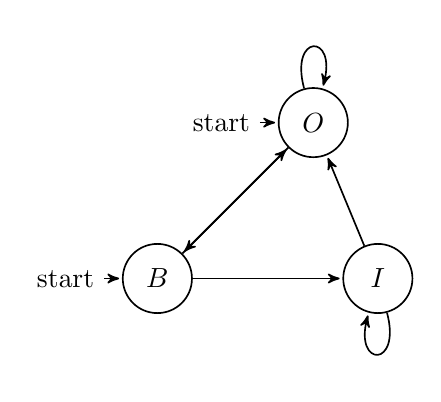
\begin{tikzpicture}[scale=0.5, ->,>=stealth',shorten >=1pt,auto,node distance=2.8cm, semithick ]
  \tikzstyle{every state}=[fill=white,draw=black,text=black]

  \node[initial,state] (A)                    {$B$};
  \node[state]         (B) [right of=A] {$I$};
  \node[initial,state]         (C) [above right of=A] {$O$};

  \path (A) edge              node {} (B)
            edge              node {} (C)
        (B) edge [loop below] node {} (B)
            edge              node {} (C)
        (C) edge [loop above]  node {} (C)
            edge               node {} (A);
\end{tikzpicture}
     \caption{\label{iobfsm} Possible states and switches for the IOB tags}
\end{figure}



\begin{table}[h]
    \begin{center}
        {\scriptsize
        \begin{tabular}{lcccccccccc}
        \hline
            \textbf{text} &We & define & a & Banach & space & as & a & complete & vector & space \\
            \textbf{POS}&PRP & VBP & DT & NNP & NN & IN & DT & JJ & NN & NN\\
            \textbf{IOB} & O& O& O& B--DFNDUM & I--DFNDUM & O& O& O& O& O \\
         \hline
    \end{tabular}
        \caption{\label{iobtags} Input example used in  training the IOB parser.}}
    \end{center} 
\end{table}

To obtain the tagged text, the whole body of text from Wikipedia was used. The examples of definitions were obtained by filtering the articles with the two following properties:
\begin{itemize}
    \item Articles that have a section with the word \textit{definition}.
    \item The title of the article must appear at least once in this section.
\end{itemize}
These sections were assumed to be definitions and the title of the article which they belong to was assumed to be the definiendum.  Only 5,229 articles were found matching this criteria (February 2019) out of the more than 6 million articles in the English Wikipedia. The dataset was split into training and test data, the results are shown in figure \ref{iobstats}. When run on the definitions found on the algebraic geometry (math.AG) articles uploaded to arXiv on 2015, the results are pictured on figure \ref{cumterms}.

\begin{figure}
    \centering
    \begin{minipage}{0.55\textwidth}
        \centering
    \includegraphics[width=0.95\textwidth]{cum_terms.png} 
        \caption{\label{cumterms}cumulative count of new and total term in the math.AG article of 2015.}
    \end{minipage}\hfill
    \begin{minipage}{0.4\textwidth}
        \centering
        {\small
        \begin{tabular}{lr}
    IOB Accuracy:  &91.1\%\\
    Precision:     &31.5\%\\
    Recall:        &67.6\%\\
    F-Measure:     &43.0\%
        \end{tabular}}
        \caption{\label{iobstats} Metrics for the IOB task using the ChunkScore function in NLTK}
    \end{minipage}
\end{figure}


Several difficulties were observed with this approach,  for instance, many of the articles from Wikipedia are about topics completely unrelated to mathematics. Also, after stripping all the wiki markup from the text some of the remaining text made no sense, this means that there was a high chance of the POS tags to be defective and hence the IOB would also be tainted. 

\begin{table}[h]
    \begin{center}
    \begin{tabular}{|p{0.7\textwidth}|c|}
        \hline
        \hline
        \textbf{Input to the Classifier} & \textbf{Result} \\
        \hline
        \hline
        Let $n \ge 1$. Recall that the \underline{\emph{lexicographic order}} $\le_l$ on $%
\mathbb{N}^n$ is defined by $v = (v_1, \ldots, v_n) \le_l (w_1, \ldots, w_n)
= w$ if and only if either $v = w$ or there is some $i$, $1 \le i \le n$,
with $v_j = w_j$, for all $j$ in the range $1 \le j < i$, and $v_i < w_i$.
        Then $\le_l$ is an \underline{\emph{admissible} order} on $\mathbb{N}^n$ in the sense of 
cite\{BWK:98\}. Indeed $\mathbb{N}^n$, together with componentwise addition
        and $\le_l$, forms a totally ordered abelian monoid. The \underline{lexicographic order}
$\le_l$ can be defined similarly on $\mathbb{Z}^n$, forming a totally
ordered abelian group.\newline
& \textbf{True Positive}\\
        \hline
        (\underline{Upper semicontinuity} of valuation) Let $f$ be a nonzero element of $k[x_1,
\ldots, x_n]$ and let $a \in k^n$. Then there exists a neighbourhood $V
\subset k^n$ of $a$ such that for all $b \in V$ $v_b(f) \le_l v_a(f)$.
& \textbf{False Positive} \\
        \hline
This claim concerns valuation-invariant lifting in relation to $P_L(A)$:
it asserts that the condition, `each element of $P_L(A)$ is valuation-invariant
in $S$', is sufficient for an $A$-valuation-invariant stack
in $\mathbb{R}^n$ to exist over $S$.
 & \textbf{True Negative}\\
        \hline
        Let $f/g$ be a nonzero element of $K$, let $U \subset k^n$ be an \underline{open set}
throughout which $g \neq 0$, and let $a \in U$. Then there exists a
neighbourhood $V \subset U$ of $a$ such that for all $b \in V$ $\mathrm{ord}%
_b(f/g) \le \mathrm{ord}_a(f/g)$.
& \textbf{False Positive}\\
        \hline
    \end{tabular}
    \caption{\label{examples}Examples of the  performance of the classifier and NER system on article  arXiv:1501.06563} The terms identified by the NER system have been underlined, the rest of the typesetting is taken verbatim from the original article.
    \end{center} 
\end{table}
 
\section{Conclusions and Future Work}
The main objective of this article is to showcase the feasability of a system that can search for definitions and important terms in large bodies of mathematical text. This system should have extremely good classification performance in order to avoid the errors propagating to the NER system. On the other hand, the system needs to be fast enough to tackle large corpora such as all the mathematical articles in the arXiv. Considering the performance of the state of the art methods for text classification and NER available today, and after observing the performance of the current prototype, we believe that this system is possible.

The next step in order to use more sophisticated methods is to use  word embeddings or language models. Methods that utilize these achieve better performance in both of the classification and NER tasks. 

In order to further better the performance of the NER subtask we also plan on increasing the amount of training data. The technique we used for the Wikipedia data can be adapted to other websites that host similar content like The Stacks Project (\texttt{https://stacks.math.columbia.edu/}) and the Groupprops subwiki (\texttt{https://groupprops.subwiki.org}). Additionally, applying  \emph{domain adaptation} methods might help to improve performance in case that the labeled data deviates significantly from nonlabeled data \cite{domainAdaptation}.


\bibliographystyle{plain}
\bibliography{cicm_article}
\end{document}
